\documentclass[a4paper]{book}
\usepackage{graphicx}
\usepackage{ragged2e}
\usepackage{xcolor}
\usepackage[nottoc]{tocbibind}
\setcounter{secnumdepth}{3}
\setcounter{tocdepth}{3}
\usepackage{amssymb,amsmath,amsthm}
\pagestyle{empty}
\usepackage{float}


\usepackage[style=authoryear,sorting=none]{biblatex}

\begin{document}
	\begin{chapter}{Development}

\tableofcontents
\newpage		
		
\section{Development of Industrial Applications: Robot Machining}
\subsection{Introduction}
CNC Machining is a process used in the manufacturing sector that involves the use of computers to control machine tools. Tools that can be controlled in this manner include lathes, mills, routers and grinders using CNC machining language (called G-code) that essentially controls all features like feed rate, coordination, location and speeds. There are many advantages to using CNC Machining. The process is more precise than manual machining, and can be repeated in exactly the same manner over and over again.
\paragraph{CNC Machine} A Conventional CNC Machine is usually designed to do only one type of manufacturing processes. For example, a 3-axis CNC Milling machine is designed to hold a spinning, multi-tooth cutter (spindle) which moves along the three cartesian coordinated to remove material to form a specific structure. This machine is mechanically built to fit the relatively slow and forceful motions required to mill through hard materials, and converting this machine to do other processes like 3d printing or laser cutting will not give the optimum output.
\paragraph{CNC Robotic Arm } Recently robots can perform the exact cuts and movements needed to produce the highest quality of milling process.Milling with a robotic arm is extremely economical; robots can be reassigned to perform other assignments in a shop - arc welding, material handling, etc. In addition, a robotic arm can handle more of the milling task without the need of human intervention. Moreover, the typical 6-axis articulated robot offers more movement flexibility than a normal milling machine; A robot can mill a complex part from multiple angles. Instead of having to reposition and re-clamp the prototype or mold, repeatedly, the robot can remain stationary. 
\subsection{State of the Art}
Many robot manufacturers have made it possible for their robots to understand G-Code lines generated from conventional CAM software. KUKA has its own package (KUKA.CNC) which you can buy for about 250 euros and install on your robot controller. If you find this package expensive, you can use CAM software that is able to export toolpaths into KRL directly like KUKA|prc, RoboDK, PowerMill, and  SprutCAM.
\vspace{.5cm}
\subsection{ Implementations }

We found it difficult to buy the KUKA.CNC package, and the other KRL exporting programs are not free and also required large amount of RAM to work generate the toolpath and check for singularities. We decided to make a postprocessor software to convert G-Code into KRL without needing any other software or packages except for the conventional CAM software, so we came up with two solutions:
\begin{itemize}
	\item 2D Solution: “Inkscape KRL Export” extension for converting vectors to KRL.
	\newline 
	\small Suitable for Writing, Drawing, Laser Cutting or engraving.
	\item \normalsize 3D Solution: “ZUKA CNC” a postprocessor tool for converting G-Codes (exported from MeshCAM and ArtCAM) to KRL
	\newline
	\small Suitable for Milling, 3D Printing, and Hot Wire Cutting. 
	
\end{itemize}
\subsubsection{2D Machining: KUKA Inkscape Extension}

An Inkscape extension, used to convert the contours of text and images in Inkscape to KRL Code to be used with KUKA KR C4 controllers. This work is based on the extension "Repetier G-Code Plugin for Inskscape" which is an open-source G-Code generator (written in Python) that takes vectors as inputs, and generates G-Code lines ready to use at conventional CNC machine. We’ve edited the extension to export KRL instead of G-Code, so that the exported file is ready to be copied and used on the KR C4 control unit.
inkscape (2).png
\begin{figure}[H]
	\centering
	\caption{KUKA Inkscape Extension}
	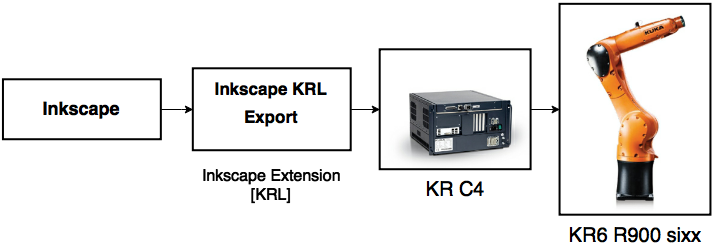
\includegraphics[width=0.8\textwidth]{ink.png}
\end{figure}

\paragraph{Adding the extension to Inkscape}
First you need to install the Inkscape software, which is free to download and use on many platforms.
To install the extension:
\begin{itemize}
	\item Go to \url{https://github.com/mnourgwad/zuka/tree/master/codes/inkscape-kuka}
	\item Download kukakrl.inx and kukakrl.py
	\item Copy the files into the extensions directory shown in the picture below.\
	\begin{figure}[H]
		\centering
		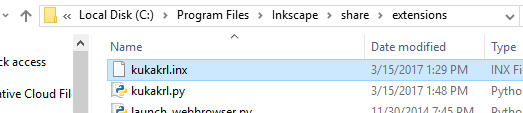
\includegraphics[width=0.8\textwidth]{0.png}
	\end{figure}
\item After a restart of Inkscape, the new extension will be available.
You can load it from Extensions \textgreater KUKA Tools \textgreater Path to KRL

\end{itemize}
\paragraph{Usage Example: Converting Text to KRL}
	
\begin{enumerate}
	\item Write your text with the text tool. The bottom left corner is the 0,0 location of the defined base or offset.
	\item Mark and position your text. If you have more objects (lines, circles, …) to embed in your KRL Code, you have to mark them all. Only marked objects will be used to generate the KRL Code.
		\begin{figure}[H]
		\centering
		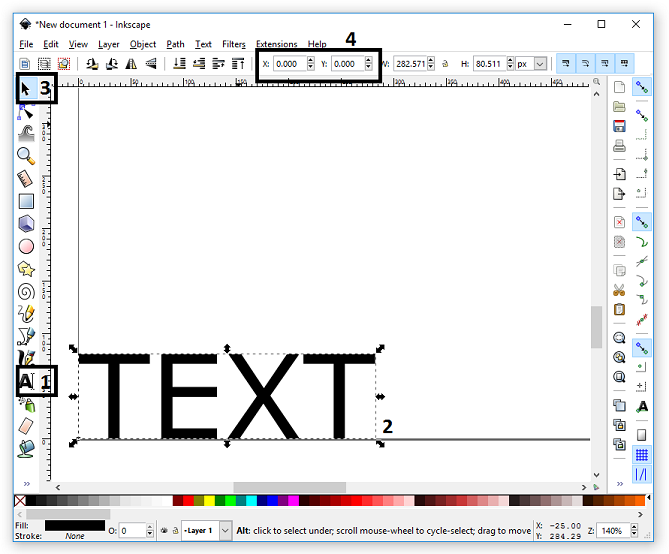
\includegraphics[width=0.8\textwidth]{1.png}
	\end{figure}
	\item Click Path \textgreater Object to Path or press Shift + Ctrl + C to convert the text into a path. The Plugin will use this path to generate the KRL Code.
	\begin{figure}[H]
		\centering
		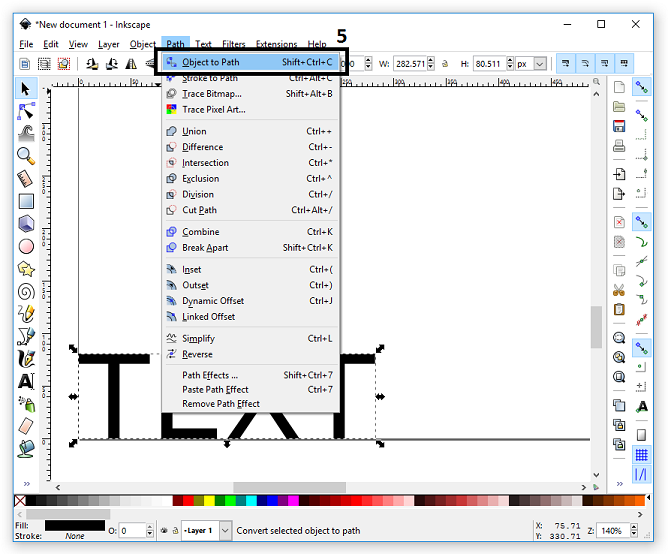
\includegraphics[width=0.8\textwidth]{2.png}
	\end{figure}
	\item Click Extensions \textgreater KUKA Tools \textgreater Path to KRL to start our plugin.
	
	\item Enter your settings.
	\item Click Apply to generate the KRL Code..
		\begin{figure}[H]
	\centering
		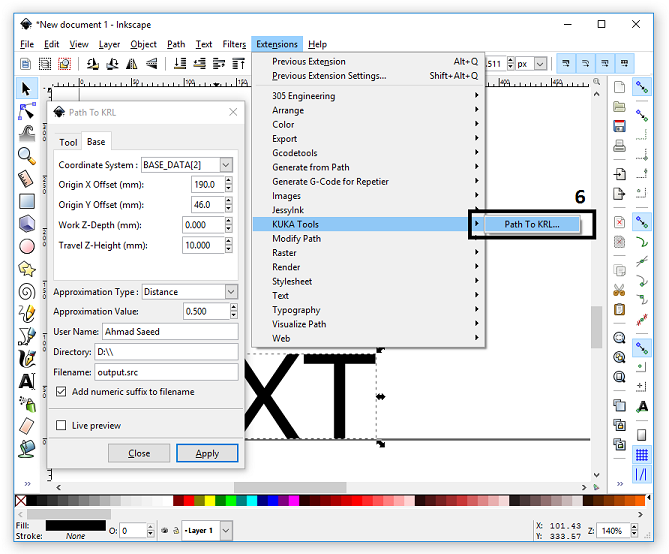
\includegraphics[width=0.8\textwidth]{3.png}
		\end{figure}
   \item After that the KRL Code will be stored and the motion path will be outlined.
   
\end{enumerate}

\paragraph{Dealing with extension settings}
\subparagraph{Tool}
Under most circumstances, a KUKA user first defines the TOOL and the BASE then refers to them in KRL using $TOOL, and $BASE system variables. The Tool can be defined through one of these two main procedures:
\begin{itemize}
	\item 	Automatically be calling the data variables created after performing any of the tool calibration processes from Start-up \textgreater Calibrate \textgreater Tool. Example: \$TOOL = TOOL\_DATA[1] where 1 is the saved tool number.
	\item Manually by entering their numeric XYZABC offset and orientation values. Example: \$TOOL = {X 280, Y 0, Z -10, A 30, B 90, C 0} where XYZ is the translational offset, and the ABC are Euler angles between the new base and the FLANGE coordinate system.
	For this extension, you can only choose the tool number that matches yours, but if you desire to write the values manually, you can edit the created SRC file and add your values.
\end{itemize}
\subparagraph{A° B° C° Orientation Angles (Euler Angles):}
Defines the relative orientation of the selected tool relative to the selected base in certain motion path. Example: LIN {X 0, Y 0, Z 0, A 90, B 180, C 0}
This transformation can be performed by:

\begin{itemize}
	\item Rotating the tool about its z-axis with an angle A (90 degrees)
	\item Rotating the tool about its y-axis with an angle B (180 degrees)
\end{itemize}
Note that the ABC angles are the same as Euler angles, but with a little bit different names, as the rotation about tool’s z-axis is named C in Euler’s.
\subparagraph{Work Speed (Feedrate)}
Defines the velocity at which the robot's TCP is moving while moving according to the desired path. It is expressed in units of Meter Per Second.
\subparagraph{Travel Speed}
Defines the velocity at which the robot's TCP is moving while jumping from a path to another. It is also expressed in units of Meter Per Second.
\subparagraph{Coordinate System}
Defines the desired Base number. The idea behind this is typically similar to the Tool
\subparagraph{Origin X, and Y Offset}
Defines the shift from the selected base origin along the x-axis and y-axis. It is expressed in millimeters.
\subparagraph{Work Z-Depth}
Defines the desired TCP's Z-axis value when the TCP is moving according to the desired path. It is expressed in millimeters.

\subparagraph{Travel Z-Height}
Defines the desired TCP's Z-axis value when the TCP is jumping from a path to another. It is expressed in millimeters.

\subparagraph{Approximation Type}
In order to increase velocity, avoid jerky motion, and achieve continuous motion along complex paths, points for which exact positioning is not necessary can be approximated. The robot takes a shortcut as illustrated 
\begin{figure}[H]
	\centering
	\caption{Approximation motion}
	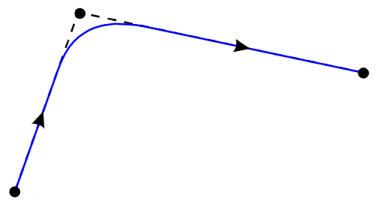
\includegraphics[width=0.8\textwidth]{approximation.png}
\end{figure}
The various approximation motions are:
\begin{enumerate}
	\item Distance: A translational distance can be assigned to the variable \$APO.CDIS. If the approximate positioning is triggered by this variable, the controller leaves the individual block contour, at the earliest, when the distance from the end point falls below the value in \$APO.CDIS. Its value is expressed in millimeters.
	\item Velocity: A percentage value can be assigned to the variable \$APO.CVEL. This value specifies the percentage of the programmed velocity \$VEL at which the approximate positioning process is started, at the earliest, in the deceleration phase of the individual block. The component which, during the motion, reaches or comes closest to the programmed velocity value, is then evaluated in terms of translation, swivel and rotation. Its value is expressed in integer number percentage.
	\item Orientation: An orientation distance can be assigned to the variable \$APO.CORI. In this case, the individual block contour is left, at the earliest, when the dominant orientation angle (swiveling or rotation of the longitudinal tool axis) falls below the angle distance, defined in \$APO.CORI, from the programmed approximate positioning point. Its value is expressed in degrees
\end{enumerate}
\textbf{Approximation Value:}
\newline
Defines the value of the selected approximation type. The greater the value of approximation, the more the path is rounded. You can get fine results by setting the its value to 0.5 for Distance type approximation
\textbf{User Name}
\newline 
Defines the name of the user making this path. It'll be added as a comment in the code's header.
\textbf{Directory}
\newline Defines the folder at which the output file will be located
\textbf{File Name}
\newline Defines the name of the output file. It should be ended with .src
\textbf{Add numeric suffix to filename}
\newline Adds a number at the end of the file name to allow multiple files with the same name to be saved in the same directory. So for instance, if the file name is output.src, it will be saved like output\_0001.src
\subsubsection{3D Machining: ZUKA CNC }
We noticed that G-Code and KRL are very similar as they consider the workspace as x y z cartesian grid, but they are different in syntax. We made “ZUKA CNC” post processing software, so that the CNC and the robot are linked to each other directly and can thus be operated like a conventional CNC controller. This tool converts conventional G-Code files into a KRL files- ready to be run on KR C4 controller.
\begin{figure}[ht]
	\centering
	\caption{ZUKA CNC blockdiagram}
	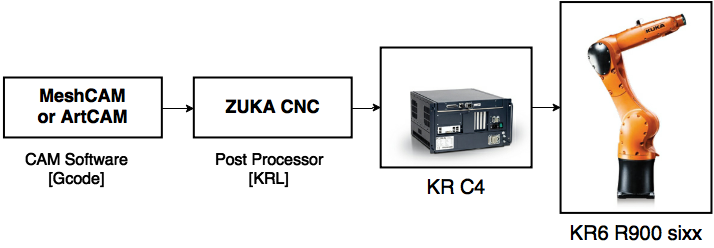
\includegraphics[width=0.8\textwidth]{zukacnc.png}
\end{figure}
For CAM processing we used Mesh CAM as it requires no previous knowledge about machining concepts. The worst part of any new CNC software is being confronted by a wall of settings to create a toolpath. MeshCAM has an Automatic Toolpath Wizard that picks as many of those values as possible so that you don't have to. You just pick the cutters, tell MeshCAM the desired quality level, and it will analyze the model to pick values to get you started. If you already know what you're doing you still have complete control over all of your toolpath settings.
\paragraph{Using MeshCAM for generating G-Code (version 6)}
\begin{itemize}
	\item From your CAD program, export the required file in STL format
	\item From MeshCAM, import the STL file from “File \textgreater Open”
	\item From MeshCAM, import the STL file from “File \textgreater Open”
	\item Choose “MM” in the dimensions window, if your file has been drawn in mm
	\item Choose “3 Axis” from the following window 
	\item Now, your model will be loaded into MeshCAM, and the left tool box options will be ready to use
	\item Use the Geometry tools for moving, scaling, and rotating your model. This is very useful as you can almost fit any model to material size by rotating and scaling.
	\begin{figure}[H]
		\centering
		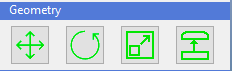
\includegraphics[width=0.8\textwidth]{11.png}
	\end{figure} 
\item -	Make sure that the origin (the intersection of x, y, and z) of the model is the same origin of your material stock. 
For this model, the origin in on the bottom left side, so the robot origin should be on the bottom left side of the material stock
\begin{figure}[H]
	\centering
	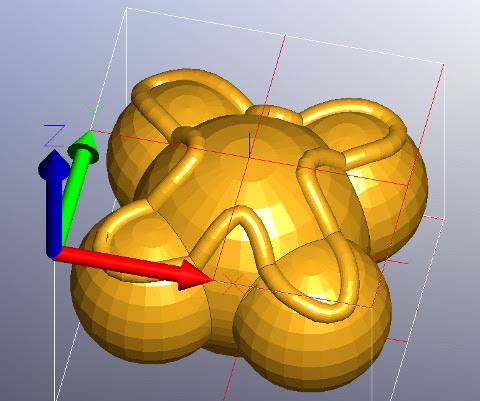
\includegraphics[width=0.6\textwidth]{22.jpg}
\end{figure} 
\item If you’re sure that all the dimensions are correct, then you are ready to Generate Toolpath. 
\begin{figure}[ht]
	\centering
	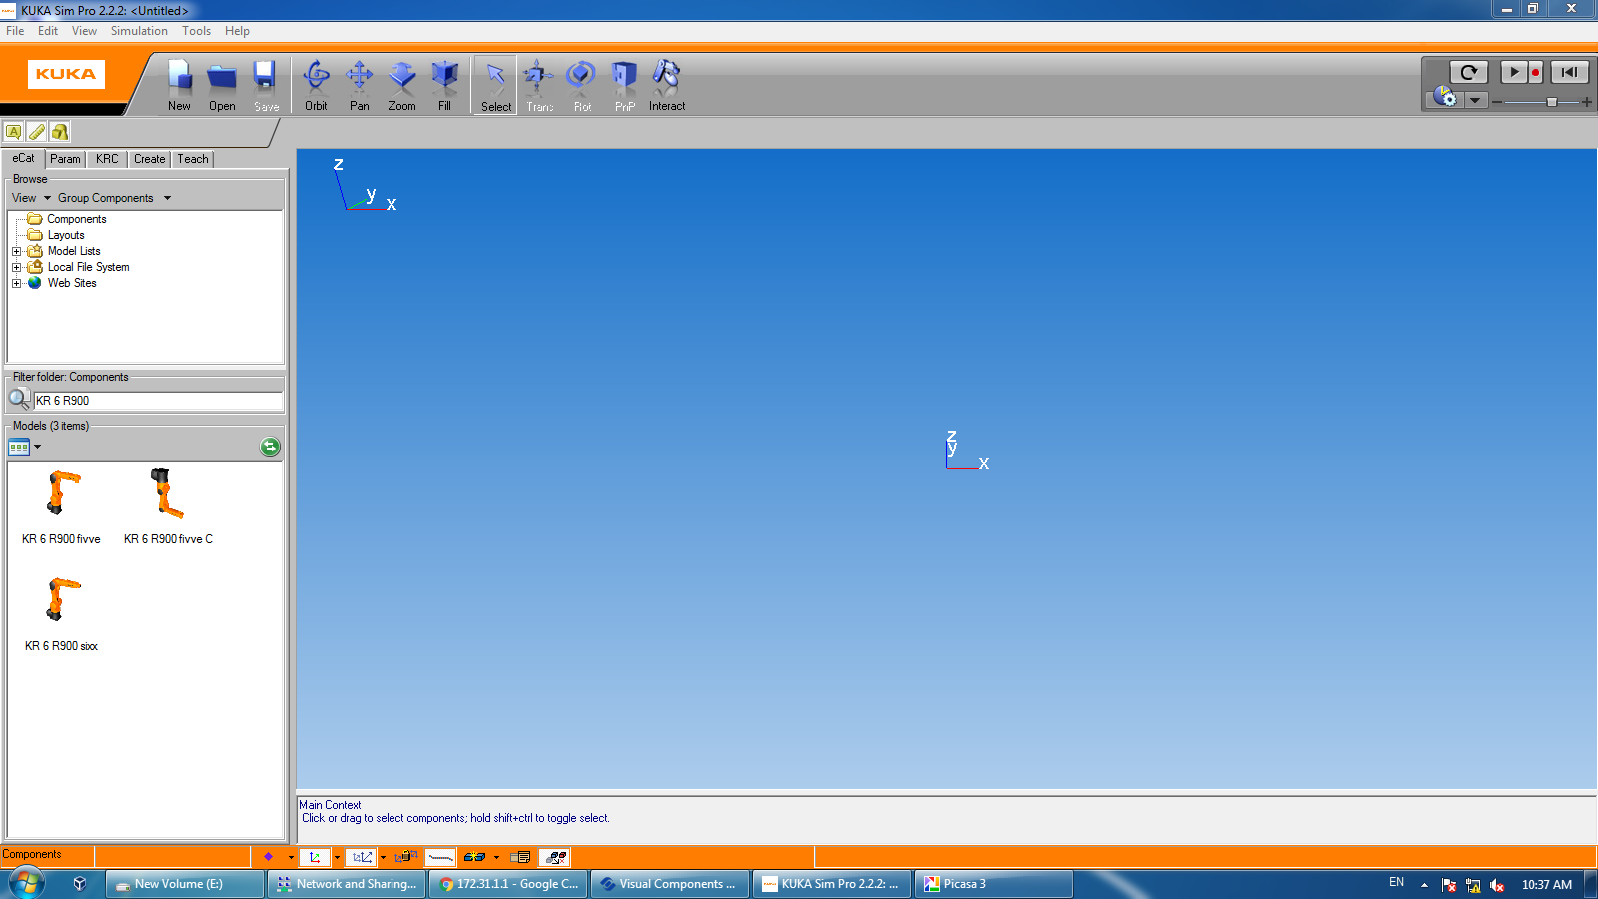
\includegraphics[width=0.6\textwidth]{33.png}
\end{figure}

\end{itemize}
Before diving into details, you should be aware of some concepts:
\begin{itemize}
	\item Roughing
	\newline
	It’s a process of quickly removing large amounts of material.  The roughing toolpath divides the geometry up into several layers to be cut in a sequence.  The result will not be satisfying as it will be rough and not containing the fine details of your model
	\item Finishing
	\newline
	It’s the process of giving the model it’s fine details and finish by moving the tool tip in more accurate and slow movements. This process is done after the roughing process
	\item Depth per Pass
	\newline
	Defines the depth of each cutting pass for the roughing toolpath. Your "depth per pass" settings can also cause bits to break. As a rule, your depth per pass should never exceed half of your bit's cutting diameter. 
	\item Stepover
	\newline
	Defines the distance between each cutting line at a given z level. A stepover of between 10\% and 20\% is typically used for finish machining toolpaths and should give a good surface finish for most materials. 
	\item Feedrate
	\newline
	Speed of cutting pass. This option will be replaced in the postprocessor with an option called “Working Speed”
	\item Plunge Rate
	Speed when plunging the tool into the stock. This option will be replaced in the postprocessor with an option called “Travel Speed”.
	
	Here is a link of the full MeshCAM options 
	\newline
	\url{http://www.grzsoftware.com/manual/toolpath_settings.htm}
	\newline
	
	You can use the Automatic Toolpath Wizard to automatically generate these options
	\begin{figure}[H]
		\centering
		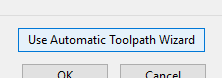
\includegraphics[width=0.6\textwidth]{44.png}
	\end{figure}


\item In order to use the Automatic Toolpath Wizard, you need only to know the dimensions of your End Mill, specially the flute length and diameter

\item From the Automatic Toolpath Wizard create a new tool and enter the dimensions of the one you’ll use, select the tolerance and quality, then let the Wizard decide the proper parameters.

\item Double check for the end mill diameter, stepover, and depth per pass 

\item Usually you don’t need the Waterline and Pencil cleanup Finish processes, so you can uncheck them.

\item Click OK and the program will hang for a minute- generating the toolpath 

\item After it finishes, click Save Toolpath As, and select “TurboCNC V3-MM” from the drop down menu, and by this point you have your G-Code file.

\item Open ZUKA CNC and load the G-Code file, convert it, and export the KRL file that you can run on your KR C4 controller

\item Please refer to the past section of the Inkscape KUKA Exporter for further details about the parameters used in this postprocessor

\item The exported program is ready to run on AUT mode. If you want to run the program on T1 mode, you should change the  
BAS(\#VEL\_PTP,10) to BAS(\#VEL\_PTP,100)

\item The operator should run a test of the program to ensure there are no problems. This trial run is referred to as "cutting air" and it is an important step because any mistake with speed, tool position, singularities, or collision could result in a scraped part.

\begin{figure}[H]
	\centering
	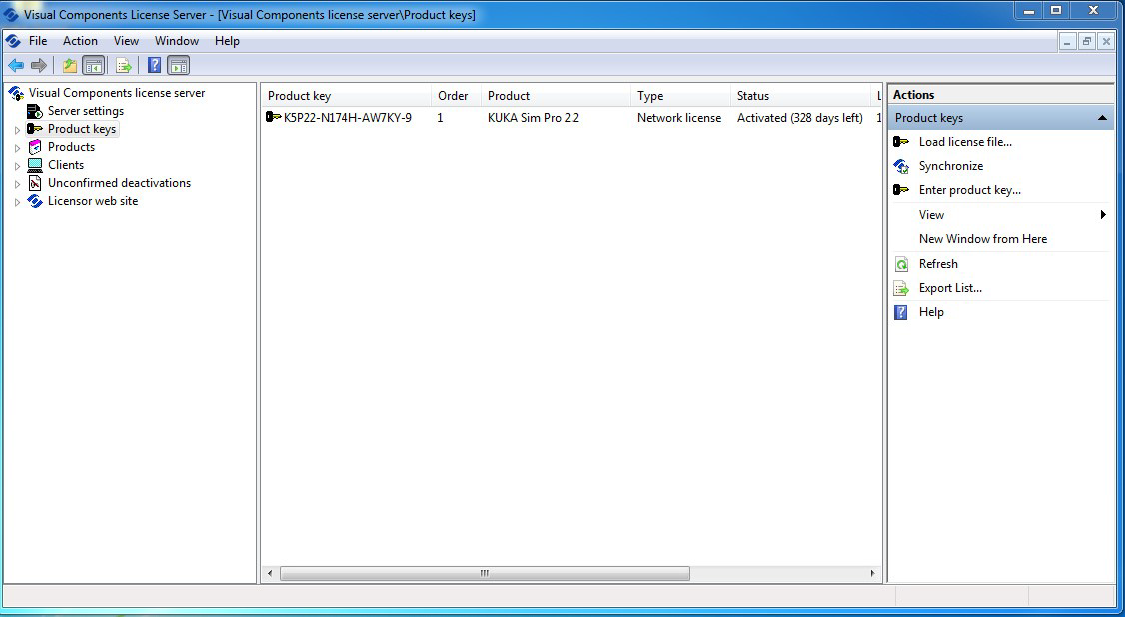
\includegraphics[width=0.9\textwidth]{55.png}
\end{figure}
	
\end{itemize}
\section{Development of KUKA communication Interface: KRL Driver}

\subsection{Introduction}
Industries that employ robots in a wide variety of applications are the main customers for robot manufacturers. The manipulator market for research applications, on the other hand, is simply too small for the robot manufacturing industry to develop models specifically for such use. 
While the hardware and mechanical requirements of developed robots are often similar for both industry and research, scientific software requirements are quite different and even contradictory in many aspects. The goal of scientist is to try to gain as much control over the robot as possible, whereas industries seek safe and easy operational interfaces.
In particular, although software interfaces that are appropriate for industrial use are available, it is difficult to find interfaces that are applicable for research purposes. The disclosure of the internal control architecture is also very hard to come by. Many manufacturers are unwilling to publish internal details regarding system architecture due to the high levels of competition in the robot market. Consequently, it is not possible to fully exploit many robotic platforms in a scientific context.

\subsection{State of the Art }
Focusing exclusively on Kuka industrial robots, the Kuka Robot Language (KRL) is the standard programming language. It is a text based language that offers data type declaration,  specification of simple motions, and interaction with tools and sensors via Input/Output (I/O) operations. It is only possible to run KRL programs on the Kuka Robot Controller (KRC), where program execution is done in accordance with real-time constraints. 
While the KRL offers an interface that is easy to use in industrial applications, it is quite limited for research purposes. In particular, the KRL is tailored to the underlying controller and consequently, only a fixed, controller-specific set of instructions is offered. Advanced mathematical tools such as matrix operations, optimization or filtering methods are not supported, thus making the implementation of novel control approaches very difficult. There is no native way to include third party libraries and as such, extending the KRL to include new instructions and functionalities is an arduous task. Moreover, it is not possible to directly use external input devices. 
The standard workaround for partially expanding the robot’s capabilities is to use supplementary software packages provided by Kuka. Some examples of such packages are the Kuka.RobotSensorInterface , which allows the manipulator motion or program execution to be influenced by sensor data, and the Kuka.Ethernet KRL XML, a module that allows the connection of the robot controller with up to nine external systems (e.g. sensors). However, several drawbacks accompany these supplementary software packages: I/O is limited, a narrow set of functions is present and major capital investments are often required to actually purchase these packages from Kuka.

To overcome these problems, an Italian company called “IMTS S.r.L.” has hacked into the KUKA KR C controller and made it possible for any device to connect through a TCP/IP protocol to read and write the values of the Global system variables. Since then, many researchers have developed interfaces for this connection like OpenShowVar and JOpenShowVar, but these tools are mainly used to track the robot variables during operation, and move it in limited ways.
\subsection{Implementation}

We started developing an open-source PC interface for KUKA robots programming. This interface makes it possible to program the robot through Python -which is a really good language in dealing with different data types, matrices, and complex calculations, and thus many applications like Artificial Intelligence, Computer Vision, and Machine Learning can be easily implemented. 
This interface is making use of the KUKAPROXYVAR proxy server, which is an TCP/IP interface to Kuka robots that allows for reading and writing variables and data structures of the controlled manipulators.
 
\subsubsection{Operation}
\begin{figure}[H]
	\centering
	\caption{KRL Driver System}
	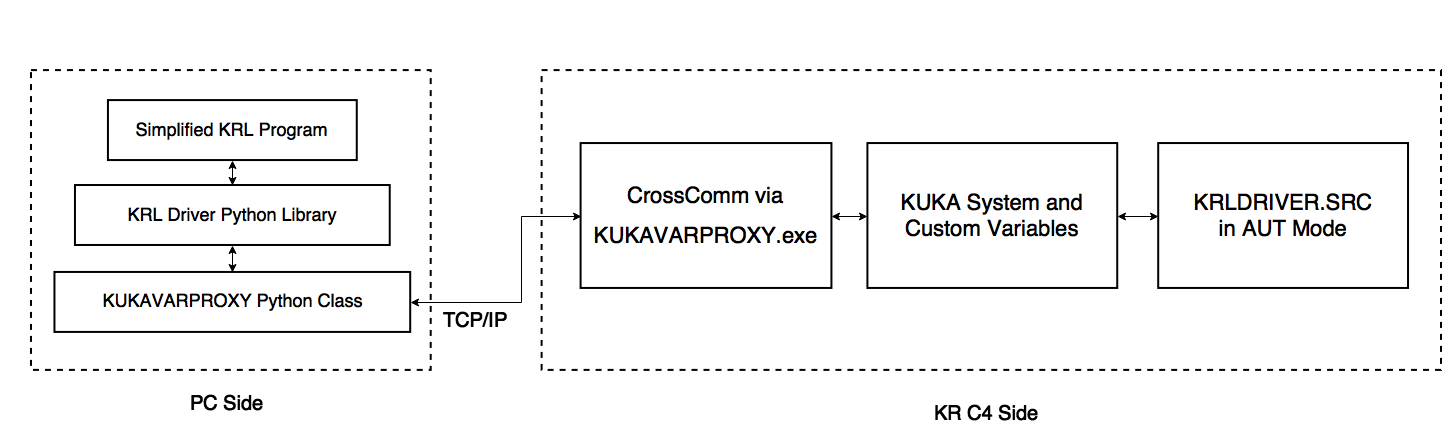
\includegraphics[width=0.6\textwidth]{krldriver.png}
	\end{figure}
	The kukavarproxy is a TCP/IP server that listens for network messages on the TCP port 7000, the reads and writes data to the KRC system variables.
	We installed the KUKAVARPROXY, created custom system variables on the KUKA side, and wrote python class and library- on the PC side- to communicate with KUKAVARPROXY to read or change the value of these variables. We also wrote a KRL program- on the KUKA side- to read these variables and act according to them. This made it possible for controlling the robot through normal python code, and opened new world of easy and flexible possibilities for users

\subsubsection{KRL Driver}
\paragraph{Usage}
The KRC robot controller runs the Microsoft Windows operating system. The teach pendant shows an “HMI” which is a program that KUKA developed to run on Windows and it is the interface that the robot user has to manipulate the robot through. In order to establish an Ethernet (TCP/IP) connection, you first need to run kukavarproxy on the controllers operating system, then configure the network connection from KUKA "HMI".
\newline \vspace{.3cm}
\textbf{You can get the libraries from}
\newline \url{https://github.com/mnourgwad/zuka/tree/master/codes/kukavarproxy-msg-format}
\subparagraph{Copying kukavarproxy to the operating system on the KRC:}
\begin{itemize}
	\item Get the kukavarproxy from: \newline  \url{https://sourceforge.net/projects/openshowvar/files/openshowvar/REV\%200.13.0/kukavarproxy-6_1.rar/download  or from https://github.com/aauc-mechlab/JOpenShowVar/tree/master/KUKAVARPROXY\%20rev\%206.1.0.101}
	\item Unpack and copy the folder to a USB flash drive
	\item Plug it to the KRC (not the teach pendant)
	\item Log in as an Expert or Administrator. For KR C4: KUKA Menu \textgreater Configuration \textgreater User Group. Default password is kuka
	\item Minimize the "HMI". For KR C4:KUKA Menu \textgreater Startup \textgreater Service \textgreater Minimize HMI
	\item Copy kukavarproxy folder to the Desktop (or anywhere else)
	\item Start the KUKAVARPROXY.exe
	\item If you have a problem with the file cswsk32.ocx, Use this command in the Administrator Command Prompt regsvr32.exe c:\\asdf\\cswsk32.ocx while changing the asdf with the true path to the file.
	\item You can make this program start automatically on reboot by creating a shortcut of KUKAVARPROXY.exe in Windows Start \textgreater All Programs\textgreater Right click Startup \textgreater Open
	
\end{itemize}
\subparagraph{HMI Network Configuration}
\begin{itemize}
	\item Connect the robot to a network. (private one is recommended) (Port X66 is used)
	\item Configure the KRC IP. For KR C4: KUKA Menu \textgreater Startup \textgreater Network Configuration
	\item Unlock port 7000. For KR C4: KUKA Menu \textgreater Startup \textgreater Network Configuration \textgreater Advanced
	\item NAT \textgreater Add Port \textgreater Port number 7000
	\item Set permitted protocols: tcp/udp
	
\end{itemize}
\paragraph{Programming from PC }
\begin{itemize}
	\item Open python (version 2.7 is recommended(
	\item Import the KRL library in your code 
	\item The default IP for the library is (172.31.1.147), so if you have a different one you should edit this from the library itself. 
	\item The next provided example shows how to use the library functions 
	\item You can edit the library and the KRLDRIVER.SRC to add any additional desired commands.
\end{itemize}
\newpage
\section{Development of Research Applications: Vision System Implementation}
\subsection{Introduction}
Robots have been blind for long time resulting to have bad impact on robot's performance and its efficiency. In our modern era of collaborative robotics, however, vision systems are becoming a necessity as we implement robots into more complex jobs and tasks.


Computer vision libraries made it possible to detect human body and hence a safe operation zone can be provided. For more applications, you can have a look at this interesting IEEE article:
\url{http://spectrum.ieee.org/automaton/robotics/diy/top-10-robotic-kinect-hacks} 

\subsection{State of the Art}

One of the most important piece of information that a normal camera misses is the depth of the image. The depth is important in recognizing the real world in a proper way. Researchers had found many solutions for this problem like the stereo camera installations, or even including depth sensors with the RGB camera itself, like in the Kinect.
Kinect is a depth sensor which is able to return images like an ordinary camera, but instead of color, each pixel value represents the distance to the point. As such, the sensor can be seen as a range- or 3D-camera. For more technical details about Kinect, please refer to this website:
\newline \url{ https://ese.wustl.edu/ContentFiles/Research/UndergraduateResearch/CompletedProjects/WebPages/fl12/MattJohnson/kinect1.html }
Robotic grasping, object recognition, and human tracking became possible by interfacing Kinect camera to robots, especially robotic manipulators.

\subsection{Implementations}
We’ve used the Kinect and Robot Operating System (ROS) platform to implement two vision dependent systems on the KUKA robot:\begin{itemize}
	\item Visual Servoing System, that makes the robot moves according to the tracked person’s hand position
	\item Safe Operating Zone, where the robot slows down to 10\% of its speed when a human is detected in the selected zone.
\end{itemize}



\subsubsection{Visual Servoing: Hand Guiding}
\paragraph {Overview}
Robotic systems can be controlled using visual data generated by means of computer vision from the workspace to do certain tasks.There are variant approaches to implement a visual servoing, one involves geometric interpretation of information captured by vision sensors, such as estimating the pose of the target and parameters of the data captured by the camera and the motion tracking system. 
\newline \vspace{.5cm}
ZuKa Hand Guiding system allows the human operator to move TCP (tool center point) along specific path using human skeleton joints. The system can be abstracted to three main layers:
\begin{itemize}
	\item Top: KUKAVAPROXY, this is a TCP/IP interface to Kuka robots that allows for reading and writing variables and data structures of the controlled manipulators to export target position to the robot in KRL format.
	
	\item  Middle : Robot Operating System -ROS- which provides communication with all system elements to analyze data captured by kinect.
	
	\item Bottom : hardware devices that capture the visual elements of the scene (Kinect XBOX 360)
\end{itemize}
\begin{figure}[H]
	\centering
	\caption{ZuKa Hand Guide System}
	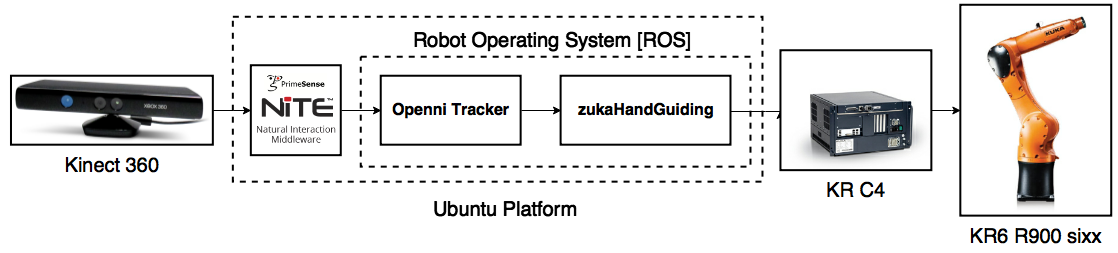
\includegraphics[width=0.8\textwidth]{88.png}
\end{figure} 

\paragraph{Usage}
\begin{enumerate}
	\item KUKA Teach Pendant Setup
	\begin{enumerate}
		\item While in Expert mode, select \textbf{R1/ KRLDRIVER.SRC}
		\item Run the program in the automatic mode.
	\end{enumerate}
\item PC Setup
\begin{enumerate}
		\item Download \textbf zukaHandGuiding
		\item Add the file to Src folder in your package( further details on creating your own package at:
		\newline	\url{http://wiki.ros.org/ROS/Tutorials/CreatingPackage}
		
		\item Make the node executable
		\item Launch kinect driver “Openni\_launch”(refer to Chapter 5 for more details)
		\item Start tracking by running openni\_tracker node
		\item Run \textbf{zukaHandGuiding} node
		
	\end{enumerate}
	
\end{enumerate}

\textbf{Download Links:}
\begin{itemize}
	\item Openni\_tracker \newline \url{
		https://github.com/mnourgwad/zuka/tree/master/codes/openni_tracker }
	
	\item	zukaHandGuiding: \newline \url{
		https://github.com/mnourgwad/zuka/tree/master/codes/zukaHandGuiding }
	\begin{figure}[H]
		\centering
		\caption{ZuKa Hand Guide System flowchart}
		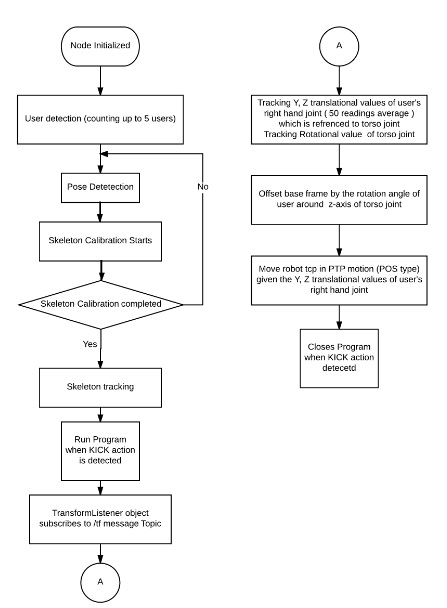
\includegraphics[width=1\textwidth]{flowchart.png}
	\end{figure} 
\end{itemize}

\newpage
\subsubsection{Safe Operating Zone}
\paragraph{Overview}
Human safety is the main concern which prevents performing some tasks requiring physical interaction between human and robot. Therefore, the safety concept was previously based on eliminating contact between human and robots.
Using vision system, we’ve made it possible for the robot to detect and recognize human body, and its distance to the fixed camera, hence a safe operating zone can be acquired by sending a signal to the robot to change its speed when a human is in the safety zone.
This is done by sending the RGB and depth data from the Kinect to the NiTE library, which is a middleware that provides body and skeleton detection, then reading this data by a ROS node to calculate the instantaneous distance of each human’s center of mass, and the signal is sent by another ROS node that listens to the stream of the least user distance.


\begin{figure}[H]
	\centering
	\caption{Zuka Safe Operation }
	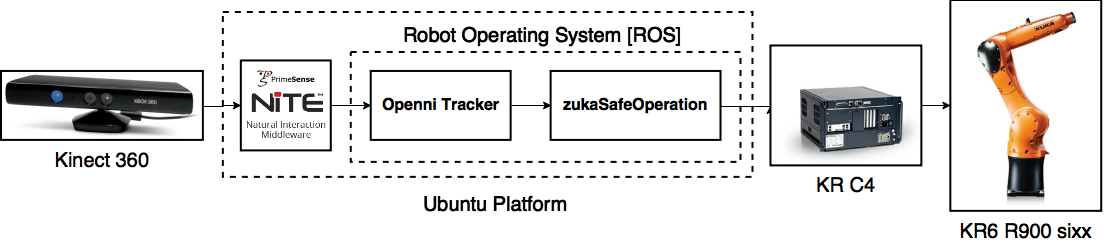
\includegraphics[width=0.8\textwidth]{7.png}
\end{figure} 
\paragraph{Usage}
Follow these steps for appropriate setup.
\begin{itemize}
	\item Install kukavarproxy as explained before, and make sure that everything is ok
	\item Install ROS, NiTE, and openni\_tracker as explained before in chapter 5
	\item Launch the roscore, but don’t launch the openni\_tracker node
	\item Copy the our modified openni\_tracker.cpp file to your catkin openni\_tracker package. Our node publish and extra topic called /closestUserDistance which gives the least detected distance of any tracked user without the need of standing in the psi calibration position
	\item Copy the zukaSafeOperation package to your catkin workspace, and run catkin\_make to build the node. Don’t forget to change node mode to executable if it hasn’t.
	\item Use: rosrun zukaSafeOperation zukaSafeOperation to launch the package
	\item The package requires a proper internet connection through kukaproxvar, and changes the robot speed to 10\% of it’s speed when a user is detected within a range of 2 meters
	
\end{itemize}

To edit the \textbf{detection data and the speed limits}:
\newline In the source code you’ll find variables to define the range, and the limited speed. Change these variables to your desired ones
\vspace{0.5cm}

\textbf{Download Links:}


\begin{itemize}
	\item Openni\_tracker \newline \url{
		https://github.com/mnourgwad/zuka/tree/master/codes/openni_tracker }
	
	\item	zukaSafeOperation: \newline \url{
		https://github.com/mnourgwad/zuka/tree/master/codes/zukaSafeOperation }
\end{itemize}
 
\end{chapter}

\end{document}